\documentclass[]{article}
\usepackage[utf8]{inputenc}
\usepackage[brazil]{babel}
\usepackage{amsthm}
\usepackage{graphicx}
\usepackage{color}
\usepackage{xfrac}
\usepackage{multicol}
\usepackage{amsthm}
\usepackage{marginnote}
\usepackage{url}
\usepackage{cancel}
\usepackage{subfigure}
\usepackage{ulem}
\usepackage{multicol}
\usepackage{amssymb}
\usepackage{adjustbox}
\usepackage{amsmath}
\usepackage{soul}
\usepackage[left=3cm,top=3cm,right=2cm,bottom=2cm]{geometry}
\usepackage[round,sort]{natbib}
\usepackage{xcolor}
% Definindo novas cores
\definecolor{verde}{rgb}{0.25,0.5,0.35}
\definecolor{jpurple}{rgb}{0.5,0,0.35}
\usepackage{listings}
\lstdefinelanguage{pseudocode}{
	keywordstyle=\bfseries\color{blue},
	keywords={function, if,then,else,while,do,end,for, to, each,in,return, true, false, talque, dobra\_strings, dobra\_strings, forca\_bruta, KNP, BMH, libera, read\_inteiro, read\_string},
	basicstyle=\small\ttfamily,
	commentstyle=\color{gray},
	mathescape=true,
	morecomment=[l]{//},
	morecomment=[s]{/*}{*/}
}
\newtheorem{definicao}{Definição}
%\lstset{
%	language=Java,
%	basicstyle=\ttfamily\small,
%	keywordstyle=\color{jpurple}\bfseries,
%	stringstyle=\color{red},
%	commentstyle=\color{verde},
%	morecomment=[s][\color{blue}]{/**}{*/},
%	extendedchars=true,
%	showspaces=false,
%	showstringspaces=false,
%	numbers=left,
%	numberstyle=\tiny,
%	backgroundcolor=\color{cyan!10},
%	breakautoindent=true,
%	captionpos=b,
%	xleftmargin=0pt,
%	tabsize=4
%}

\begin{document}
	
	
%cabecalho
\begin{figure}[t]
	\centering
	
\includegraphics[width=2.5cm]{ufsj}\\
	
	{\large Universidade Federal de São João del Rei\\
		Departamento de Ciência da Computação\\
		Curso de Ciência da Computação\\}
	\label{fig:ufsj}
\end{figure}
{\Large
	\begin{center}
		%Modelo de Documentação para enfrentar $\vec{A} E \mathbb{D} \Sigma^3$
		\textbf{Trabalho Prático 1: utilização de métodos numéricos na implementação de uma rede neural para classificação de imagens}
		
	\end{center}
}

{\large 
	
	\begin{center}
		Adelson de Oliveira Carmo Júnior, 
		Henrique Hott,
		Luiz Filipe Almada, \\
		Luiz Filipe Magalhães,
		Rodrigo José Zonzin Esteves
	\end{center}	
}
\section{Problema a ser resolvido}

\section{Modelagem de Redes Neurais}
De acordo com \cite{haykin}, uma rede neural é um modelo matemático de processamento dados  dotado das seguintes propriedades: \textit{não linearidade, mapeamento de entrada/saída, adaptatividade e capacidade de generalização}. 



\subsection{Neurônios}
A unidade mais elementar de uma rede neural é um neurônio. Temo a seguinte representação: 
\begin{figure}[h!]
	\centering
	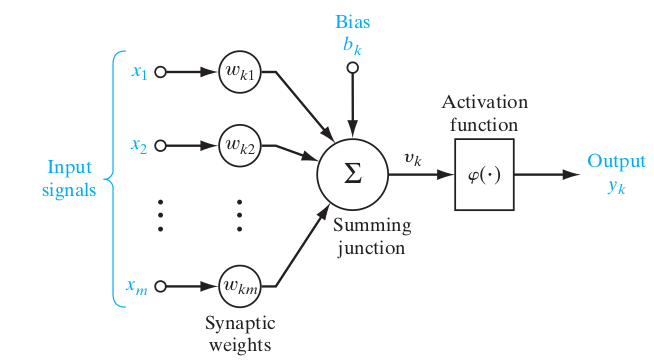
\includegraphics[width=0.5\linewidth]{imagens/neuronio}
	\caption{Representação matemática de um neurônio}
	\label{fig:neuronio}
\end{figure}

Um neurônio: 
\begin{enumerate}
	\item Recebe um vetor de entrada dados: $X = x_1, x_2, \ ... \ , x_n$
	\item Multiplica elemento a elemento do vetor de dados por um vetor de pesos $W = w_1, x_2, \ ... \ , w_n$
	
	\item Faz a soma dos $n$ produtos obtidos no passo anterior.
	$ x_1w_1 + x_2w_2 + ... + x_nw_n$. 
	Esse procedimento, nada mais é do que o produto interno dos vetores $X$ e $W$. Pode-se somar um vetor $b$ de $bias$. 
	$$< X, W > = \sum x_i w_i$$
	
	\item Função de ativação $\phi$: aplicação de uma função \textbf{não linear}. 
	É importante que a função seja não linear pois várias camadas de neurônios serão encadeadas. Se todas as funções fossem lineares, a rede neural consistiria de um modelo linear em si. Exemplo. Sejam $f(x) = 3x +4$ e $g(x) = 2x$.
	$$f \circ g (x) = 3(2x) + 4 \Rightarrow f(x) \circ g(x) = 6x + 4$$ 
	
	Algumas funções não lineares comumente usadas: 
	$$ReLU(z) = \begin{cases}
		z, & z < 0 \\
		0, & z \geq 0 \\
	\end{cases}$$
	
	$$softmax(z) = \frac{e^z_i}{\sum_{j = 1}^{K} e^{z_j}}$$
	
	\item Portanto, para determinado neurônio $i$ temos o seguinte processamento: 
	
	$$y_i(X) = \phi(<X, W_i> + b)$$
	
\end{enumerate}

\subsection{Processo de aprendizado}
No comportamento biológico, quando um neurônio ativa outro, a conexão sináptica entre eles torna-se mais forte. \textit{``Cells that fire together, wire together}. 

Nesse sentido, quanto mais um neurônio acertar a predição de um dado, mais forte a conexão entre ele e seu sucesso deve ser. Essa conexão é mapeada pelo vetor de pesos $W$. De forma geral, o processo de aprendizado de uma rede neural consiste em computar quais valores de $W$ otimizam o acerto da rede. 

Exemplo: na regressão linear a seguir, o processo de aprendizado deve procurar quais valores $\theta_0$ e $theta_1$ representam o melhor ajuste da reta. 
$$\hat{y}(x)= \theta_0 + \theta_1x$$ 

\begin{figure}[h!]
	\centering
	
	\subfigure[Possíveis valores]{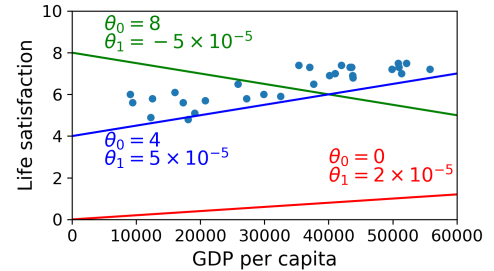
\includegraphics[width=0.4\linewidth]{imagens/aprendiado_reta}}
	\subfigure[Valores ótimos]{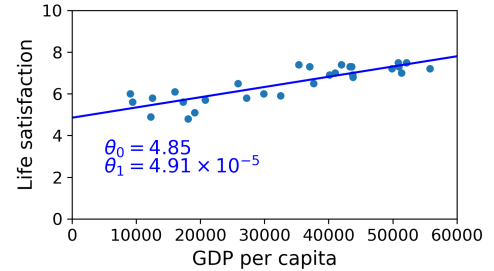
\includegraphics[width=0.4\linewidth]{imagens/aprendiado_reta_otimo}}
	
	\caption{Aprendizado do modelo $\hat{y}$}
	\label{fig:aprendiadoreta}
\end{figure}

Para cada neurônio de saída que produz uma predição errada, a conexão é reforçada alterando-se os pesos das entradas que teriam produzido uma predição correta. A regra pode ser descrita pela equação a seguir: 
$$w'_{i,j} = w_{i,j} + \eta(y_j - \hat{y}_j)x_i$$

onde $w_{i,j}$ é a conexão entre o i-ésimo neurônio de entrada e o j-ésimo de saída, $x_i$ é o $i^{th}$ valor de treinamento, $\hat{y}_j$ é a predição do neurônio $j$, $y_j$ é o valor esperado e $\eta$ é a taxa de aprendizado.   \\


De forma geral, o que essa equação faz é atualizar os pesos de um neurônio em função do erro $y - \hat{y}$, ou seja, do valor esperado com o valor predito.  

\newpage

\section{Construção do modelo}
\subsection{Preliminares}
Para a implementação do trabalho, utilizaremos a base de dados MNIST, que é constituída por imagens grayscale de dígitos manuscritos com dimensão $28 \times 28$. 

\begin{figure}[h!]
	\centering
	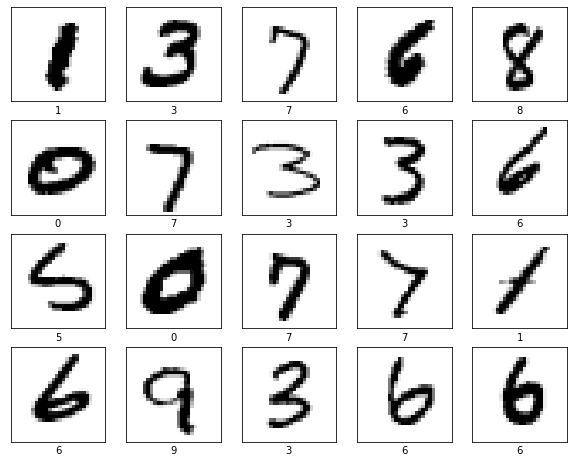
\includegraphics[width=0.4\linewidth]{imagens/mnist}
	\caption{Base de dados}
	\label{fig:mnist}
\end{figure}

Dada uma imagem $x$, nosso modelo deverá ser capaz de gerar uma resposta $f(x)$ discriminando um dos 10 possíveis dígitos.
$$f: 28 \times 28 \mapsto \{0, 1, 2, \ ... \ , 9\}$$

Cada imagem será representada por um vetor de $28 \times 28 = 784$ valores inteiros entre 0 (completamente preto) e 255 (pixel completamente branco).  Dessa maneira:

$$img = (0, 0, 0, 1, 255, \ ... \ , 0, 124)$$

\subsection{Detalhamento}
$X^T$ é uma matriz onde cada linha representa uma imagem. Para passarmos pela rede, precisamos que cada imagem seja uma coluna da matriz. Logo, usamos a transposta. 
$$X = \begin{bmatrix}
		\ldots\ldots  x^{(1)}  \ldots\ldots \\
		\ldots\ldots  x^{(2)} \ldots\ldots \\
		\vdots  \\
		\ldots\ldots  x^{(n)}  \ldots\ldots \\
	  \end{bmatrix} ^T 
	  =
	  \begin{bmatrix}
	  	\vdots & \vdots &  & \vdots \\
	  	x^{(1)} & x^{(2)} & \ldots & x^{(n)} \\
	  	\vdots & \vdots &  & \vdots \\
	  \end{bmatrix}
	  $$

\subsubsection{Forward Propagation}

Como cada imagem tem $784$ valores, precisamos de 784 nós na camada de entrada da rede. Cada nó receberá o valor de um pixel, fará o processamento e entregará um valor discriminante para uma camada escondida: 10 nós (um para cada classe). 

\begin{figure}[h!]
	\centering
	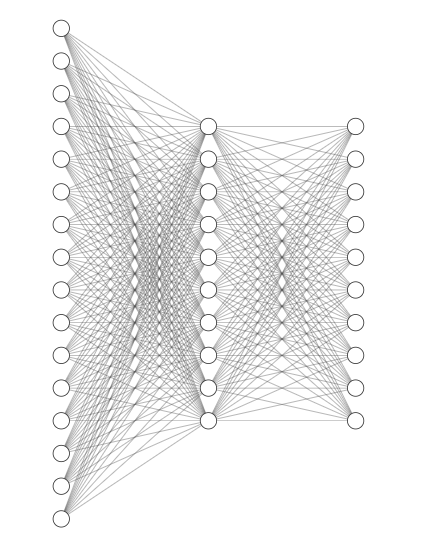
\includegraphics[width=0.3\linewidth]{imagens/rede}
	\caption{Exemplo da rede neural}
	\label{fig:rede}
\end{figure}

A camada de saída produzirá um vetor com 10 valores (0 até 9). Aquele que for mais ativado será o valor que a rede julgou como pertencente à determinada classe (reveja a função ReLU).

\begin{definicao}
A primeira camada será denotada pela matriz $A^0$, a segunda pela camada $A^1$ e a última pela camada $A^2$. 
De maneira similar, o resultado do processamento de cada camada $i$ será representado pela matriz $Z^{i}$.
\end{definicao} 

$$ A^0 = X (784 \times m)$$ 
$$ Z^1 = \ <W^1, A^0> + b^1  $$
$dim(Z^1) = \left[10 \times 784\right]  \cdot \left[ 784 \times m\right]  + \left[ 10 \times 1\right]  = 10 \times m$
$$A ^1 = ReLU(Z^1)$$
$$Z^2 = <W^2, A^1> + b^2$$
$dim(Z^2) = \left[ 10 \times 10\right]\cdot \left[ 10\times m \right]  + \left[ 10 \times 1\right] =  10 \times m$
$$A^2 = softmax(Z^2)$$
$A^2 \in \mathbb{R}^1 $

Portanto, nosso modelo $f$ é dado por 

$$f(X) = softmax(W_2 ReLU(W_1 X^T + b^1) + b^2)$$\footnote{Cuidado pra não confundir. Aqui $^T$ representa a notação do Haykin para produto interno e não a matriz transposta}

\subsubsection{Back Propagation}
O passo anterior é capaz de gerar uma resposta. Quando passamos uma imagem pela rede ele é capaz de dizer se ela é 0, 1, 2 ou \textit{whatever}. 

Mas como a rede sabe que acertou e como ela sabe quais (e quanto) pesos de $W^1$ e $W^2$ ele deve ajustar?

Ela pega a predição gerada e volta nó a nó da rede perguntando ``Eu acertei? Eu acertei?". Se sim, ela fica feliz e é isso. 

Caso contrário, ela deve calcular os pesos da seguinte forma: 
Antes começamos de $A^0$ e fomos até $A^2$. Agora vamos de $A^2$ para trás.  

$$dZ^2 = A^2 - Y$$
$dim(dZ^2) = \left[  10\times m \right]  $
$$dW^2 = \frac{1}{m}dZ^2A^{1T}$$
$dim(dW^2) = \left[ 10 \times m\right] \cdot \left[ m \times 10 \right]  = [10 \times 10 ]$
$$db^2 = \frac{1}{m}\sum dZ^2$$
$$dZ^1 = W^2dZ^2 \cdot g'(Z^1)\footnote{$g'(x) = ReLU'(x)$}$$
$dim(dZ^1) = [10 \times 10] \cdot [10 \times m] + [10 \times m] = [10 \times m]$
$$dW^1 = \frac{1}{m} dZ^1 X^T$$
$dim(dW^1) = [10 \times m] \cdot [m, 784] = [10 \times 784]$
$$db^2 = \frac{1}{m} \sum dZ^1$$

Depois de calculados os fatores de correção, devemos atualizar o vetor de fato: 

$$W^1 = W^1 - \alpha dW^1$$
$$b^1 = b^1 - \alpha db^1$$

$$W^2 = W^2 - \alpha dW^2$$
$$b^2 = b^2 - \alpha db^2$$

onde $\alpha = $ learning rate/taxa de aprendizado. Essa equação é a mesma relacionada com a figura 2. Géron chamou alfa de $\eta$. 

\textbf{O que são esses diferenciais?} 

Para otimizar os parâmetros de cada nó, é preciso achar o valor mínimo da função de custo (a função que computa o erro) e então atualizar os valores do vetor de peso. 

Uma técnica intuitiva para obter valores mínimos é achar os pontos do domínio cuja derivada é igual a zero. {\tiny \sout{$f(x) = x^3$}} 


\textit{``The basic idea is to efficiently compute partial derivatives of an approximating function $F(w, x)$ realized by the network with respect to all	the elements of the adjustable weight vector w for a given value of input vector x."} \\


O Gradiente Descendente é um método numérico para melhorar o desempenho dessa busca. Ele inicia em valores aleatórios e então caminha iterativamente em direção aos zeros da função de perda.\\ 

Observação: Em uma função $f(x, y)$, o gradiente $\nabla f(x,y)$ indica direção e sentido onde há mais incremento na função $f$. Como queremos minimizar, tomamos o sentido oposto. 

\textit{Se tá crescendo pra cá, eu vou pra lá!}\\


No nosso caso, a função de perda trabalha apenas sobre uma variável: logo $\nabla f(x) = (\frac{\partial}{\partial x} f(x) )= (\frac{d}{dx}f(x)) $. Dessa maneira, temos derivadas ordinárias em todos os termos. 

\begin{figure}[h]
	\centering
	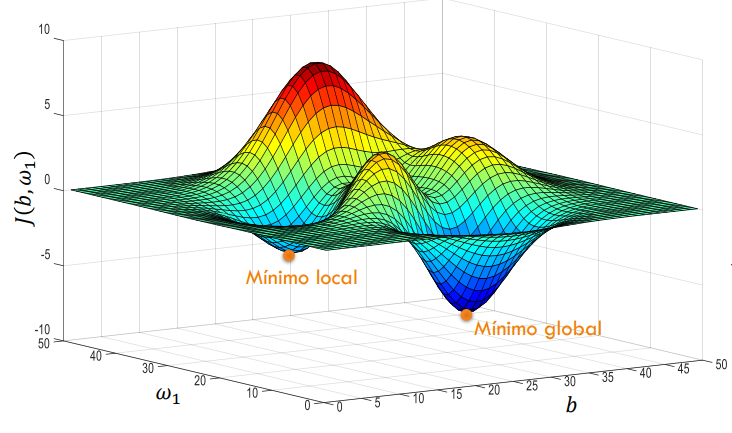
\includegraphics[width=0.4\linewidth]{imagens/gradiente}
	\caption{Vetor Gradiente Descendente}
	\label{fig:gradiente}
\end{figure}







\newpage


\bibliographystyle{apalike}
%\bibliographystyle{authordate1}
%\bibliography{referencia.bib}

\end{document}